\documentclass[]{article}



\usepackage{graphicx,forloop,caption,subcaption,float,hyperref,arrayjob,listings,color,booktabs,mathtools}
\usepackage{pdfpages}
\usepackage[margin=1.2in]{geometry}
\usepackage{amsmath}
\usepackage{multirow}
%vhdl code
\definecolor{dkgreen}{rgb}{0,0.6,0}
\definecolor{gray}{rgb}{0.5,0.5,0.5}
\definecolor{mauve}{rgb}{0.58,0,0.82}

\DeclareMathOperator*{\argmin}{\arg\!\min}


\lstset{frame=tb,
  language=VHDL,
  aboveskip=3mm,
  belowskip=3mm,
  showstringspaces=false,
  columns=flexible,
  basicstyle={\small\ttfamily},
  numbers=none,
  numberstyle=\tiny\color{gray},
  keywordstyle=\color{blue},
  commentstyle=\color{dkgreen},
  stringstyle=\color{mauve},
  breaklines=true,
  breakatwhitespace=true
  tabsize=3
}

%matlab code
\lstset{frame=tb,
  language=Matlab,
  aboveskip=3mm,
  belowskip=3mm,
  showstringspaces=false,
  columns=flexible,
  basicstyle={\small\ttfamily},
  numbers=none,
  numberstyle=\tiny\color{gray},
  keywordstyle=\color{blue},
  commentstyle=\color{dkgreen},
  stringstyle=\color{mauve},
  breaklines=true,
  breakatwhitespace=true
  tabsize=3
}


% Title Page
\title{UCLA\\EE230B\\Digital Communication Design Project\\Step 1 Report}
\author{Alican Salor 404271991 \\  \href{mailto:alicansalor@ucla.edu}{alicansalor@ucla.edu} \\ \\
Darren Reis 804359840 \\
\href{mailto:darrer.r.reis@gmail.com}{darren.r.reis@gmail.com} }


\begin{document}
\maketitle

\newpage
\tableofcontents

\newpage


\section{System Setup}
\label{sec:setup}
The system is as shown in Figure BLAH.  To simulate the system, code was written for each block in the diagram.  A random bit generator was used to output a stream of data (Appendix~\ref{app:random_bit_generator}).  The data stream then was passed into a bit-to-symbol mapper, transformed differently based on the modulation scheme (Appendix~\ref{app:bittosym}).  Various schemes were used, including Binary Phase Shift Keying [BPSK], Quadrature Phase Shift Keying [QPSK], and Quadrature Amplitude Modulation [QAM], as shown in Appendices~\ref{app:bpsk_mod}~$-$~\ref{app:qam_64_mod}. To approximate a real system:

\begin{itemize}
\item The system got passed through a square root raised cosine pulse (Appendix~\ref{app:sqrt_raised_cosine}) which has the following impulse response:

 \[
 h(t) = \begin{dcases*}
        1-\beta+4\frac{\beta}{\pi} &  $t = 0$\\         
         \\ 
        \end{dcases*}
\]

\item This filter was then oversampled by four in order to DO BLAH (Appendix~\ref{app:impulse_train}).
\item Furthermore it was broadcast over an Additive White Gaussian Noise (AWGN) channel. (Appendix~\ref{app:awgn_channel}). This channel modeled the transmission of the signal from transmitter to receiver. The variance of this channel is determined by the SNR values picked at the beginning of each simulation. In order to achieve this the following equation is used:

$\sigma^2 = S/(10^{SNR/10})$

where S is the average signal power of the chosen modulation scheme.

\item Then at the receiver a matched filter is used for optimal detection of the transmitted signal. As square root raised cosine pulse is used at the tranmission side (which a real symmetric pulse), the same square root raised cosine pulse shape is used as the matched filter.  

\item After sampling the symbol stream back at the original symbol rate, the message is ready for recovery (Appendix~\ref{app:sampler}).

\item Finally, the data waveform is sent through a decision block, demodulating according to the appropriate scheme (Appendices~\ref{app:bpsk_demod}~$-$~\ref{app:qam_64_demod}).

\end{itemize}

An analysis of performance of the system was determined by comparing a theoretical error rate to experimental bit error rate for various schemes.  The theoretical derivation is shown in Section~\ref{sec:deriv}. On the other hand the experimental error rate was found by counting the instances of wrongly decoded symbols (or bits as in BPSK case) and diving this number by the number of total symbols sent through the channel.  

\newpage
\section{Mathematical Derivations of Probability of Error}
\label{sec:deriv}
As equiprobable bits are generated and passed through an AWGN channel in this project, the have used ML decision rule which states: \\

$\hat{m} = \argmin_{1\leq m \leq M}{||\underline{r} - \underline{s}_m||}$ 
\\

Thus in the following subsections the probability of error for each constellation used in the project is derived using the minimum distance rule.

Furthermore the formulas are used to convert the minimum distance to the average bit energy and the average symbol energy to average bit energy in the M-QAM constellations:\\

$d_{min} = \sqrt{\frac{6log_2M}{M-1}E_{bavg}} $\\

$E_{bavg} = \frac{E_{savg}}{log_2M}$



\subsection{BPSK}
\label{sec:bpsk}
The exact probability of bit error is as follows (no interesting decision regions):\\

$ P_e = Q(\frac{d_{min}/2}{\sqrt{N_o/2}}) $ \\
\\
$ P_e = Q(\sqrt{2\frac{E_b}{N_o}}) $ \\

\subsection{QPSK}
\label{sec:qpsk}

The exact probability of bit error is as follows (found by subtracting the interesting decision regions from the nearest neighbor approx.):\\

$ P_e = 2Q(\frac{d_{min}/2}{\sqrt{N_o/2}})-Q(\frac{d_{min}/2}{\sqrt{N_o/2}})^2$ \\
\\
$ P_e = 2Q(\sqrt{2\frac{E_{bavg}}{N_o}})-Q(\sqrt{2\frac{E_{bavg}}{N_o}})^2$ \\

\subsection{16-QAM}
\label{sec:qam16}

The exact probability of bit error is as follows (found by subtracting the interesting decision regions from the nearest neighbor approx.):\\

$ P_e = 3Q(\frac{d_{min}/2}{\sqrt{N_o/2}})-(9/4)Q(\frac{d_{min}/2}{\sqrt{N_o/2}})^2$ \\
\\
$ P_e = 3Q(\sqrt{\frac{4}{5}\frac{E_b}{N_o}})-(9/4)Q(\sqrt{\frac{4}{5}\frac{E_{b}}{N_o}})^2$  \\

\subsection{64-QAM}
\label{sec:qam64}
The exact probability of bit error is as follows (found by subtracting the interesting decision regions from the nearest neighbor approx.):\\

$P_e = (7/2)Q(\frac{d_{min}/2}{\sqrt{N_o/2}}) -(49/16)Q(\sqrt{\frac{d_{min}/2}{\sqrt{N_o/2}}})^2$ \\

$P_e = (7/2)Q(\sqrt{\frac{18}{63}\frac{E_b}{N_o}})-(49/16)Q(\sqrt{\frac{18}{63}\frac{E_b}{N_o}})^2$ \\



\section{Step 1 Results}

In the following sections the probability of bit error versus the signal to noise ratio and scatter plots for BPSK, QPSK, 16-QAM and 64-QAM constellations .

\subsection{Probability of Error vs SNR plots}
In the sections given below considering BPSK, QPSK, 16-QAM and 64-QAM constellations the following  are plotted using the matlab functions given in the appendix:
\begin{itemize}
\item Theoretical Bit Error Rate/Symbol Error Rate curve as a function of the symbol SNR
\item The theoretical Bit Error Rate/Symbol Error Rate curve as a function of $E_b/N_o$
\item The Bit Errote Rate/Symbol Error Rate curve from the simulation as a function of the received signal's SNR
\end{itemize}

\subsubsection{BPSK}
\begin{figure}[H]
\centering
\hspace*{-2cm}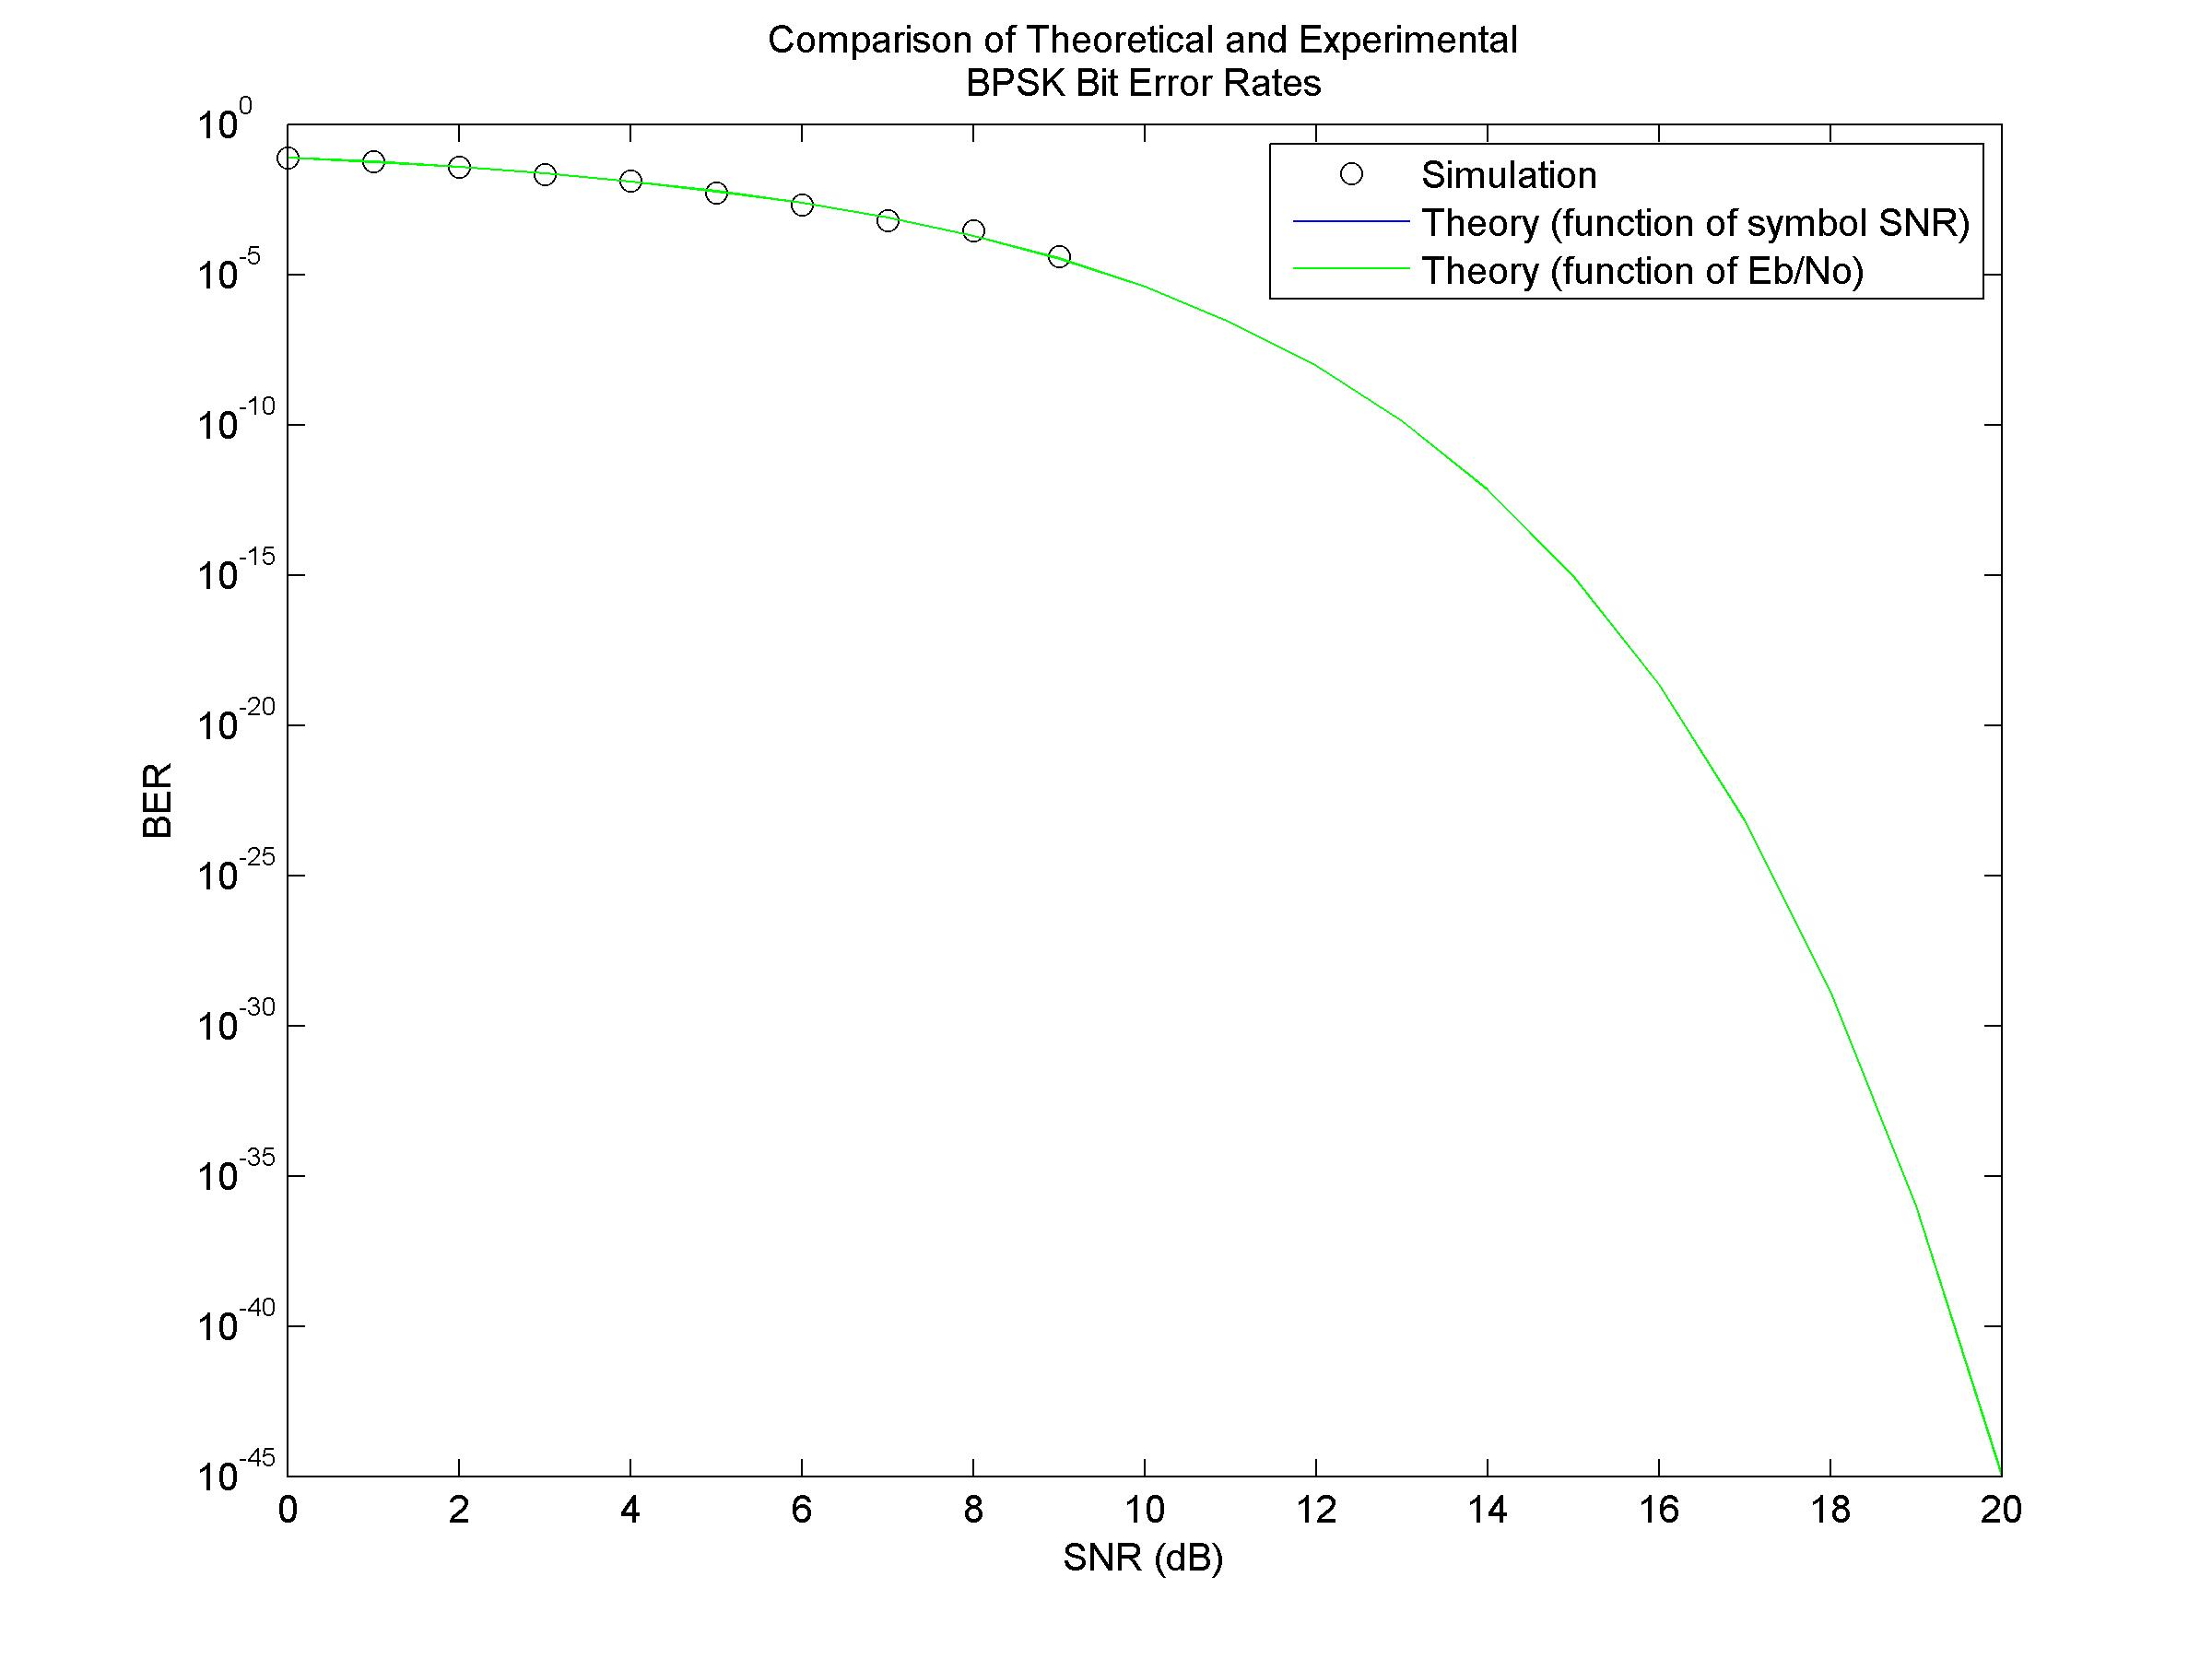
\includegraphics[width=1.3\textwidth]{bpSNR.jpg}
\caption{}
\end{figure}
\subsubsection{QPSK}
\begin{figure}[H]
\centering
\hspace*{-2cm}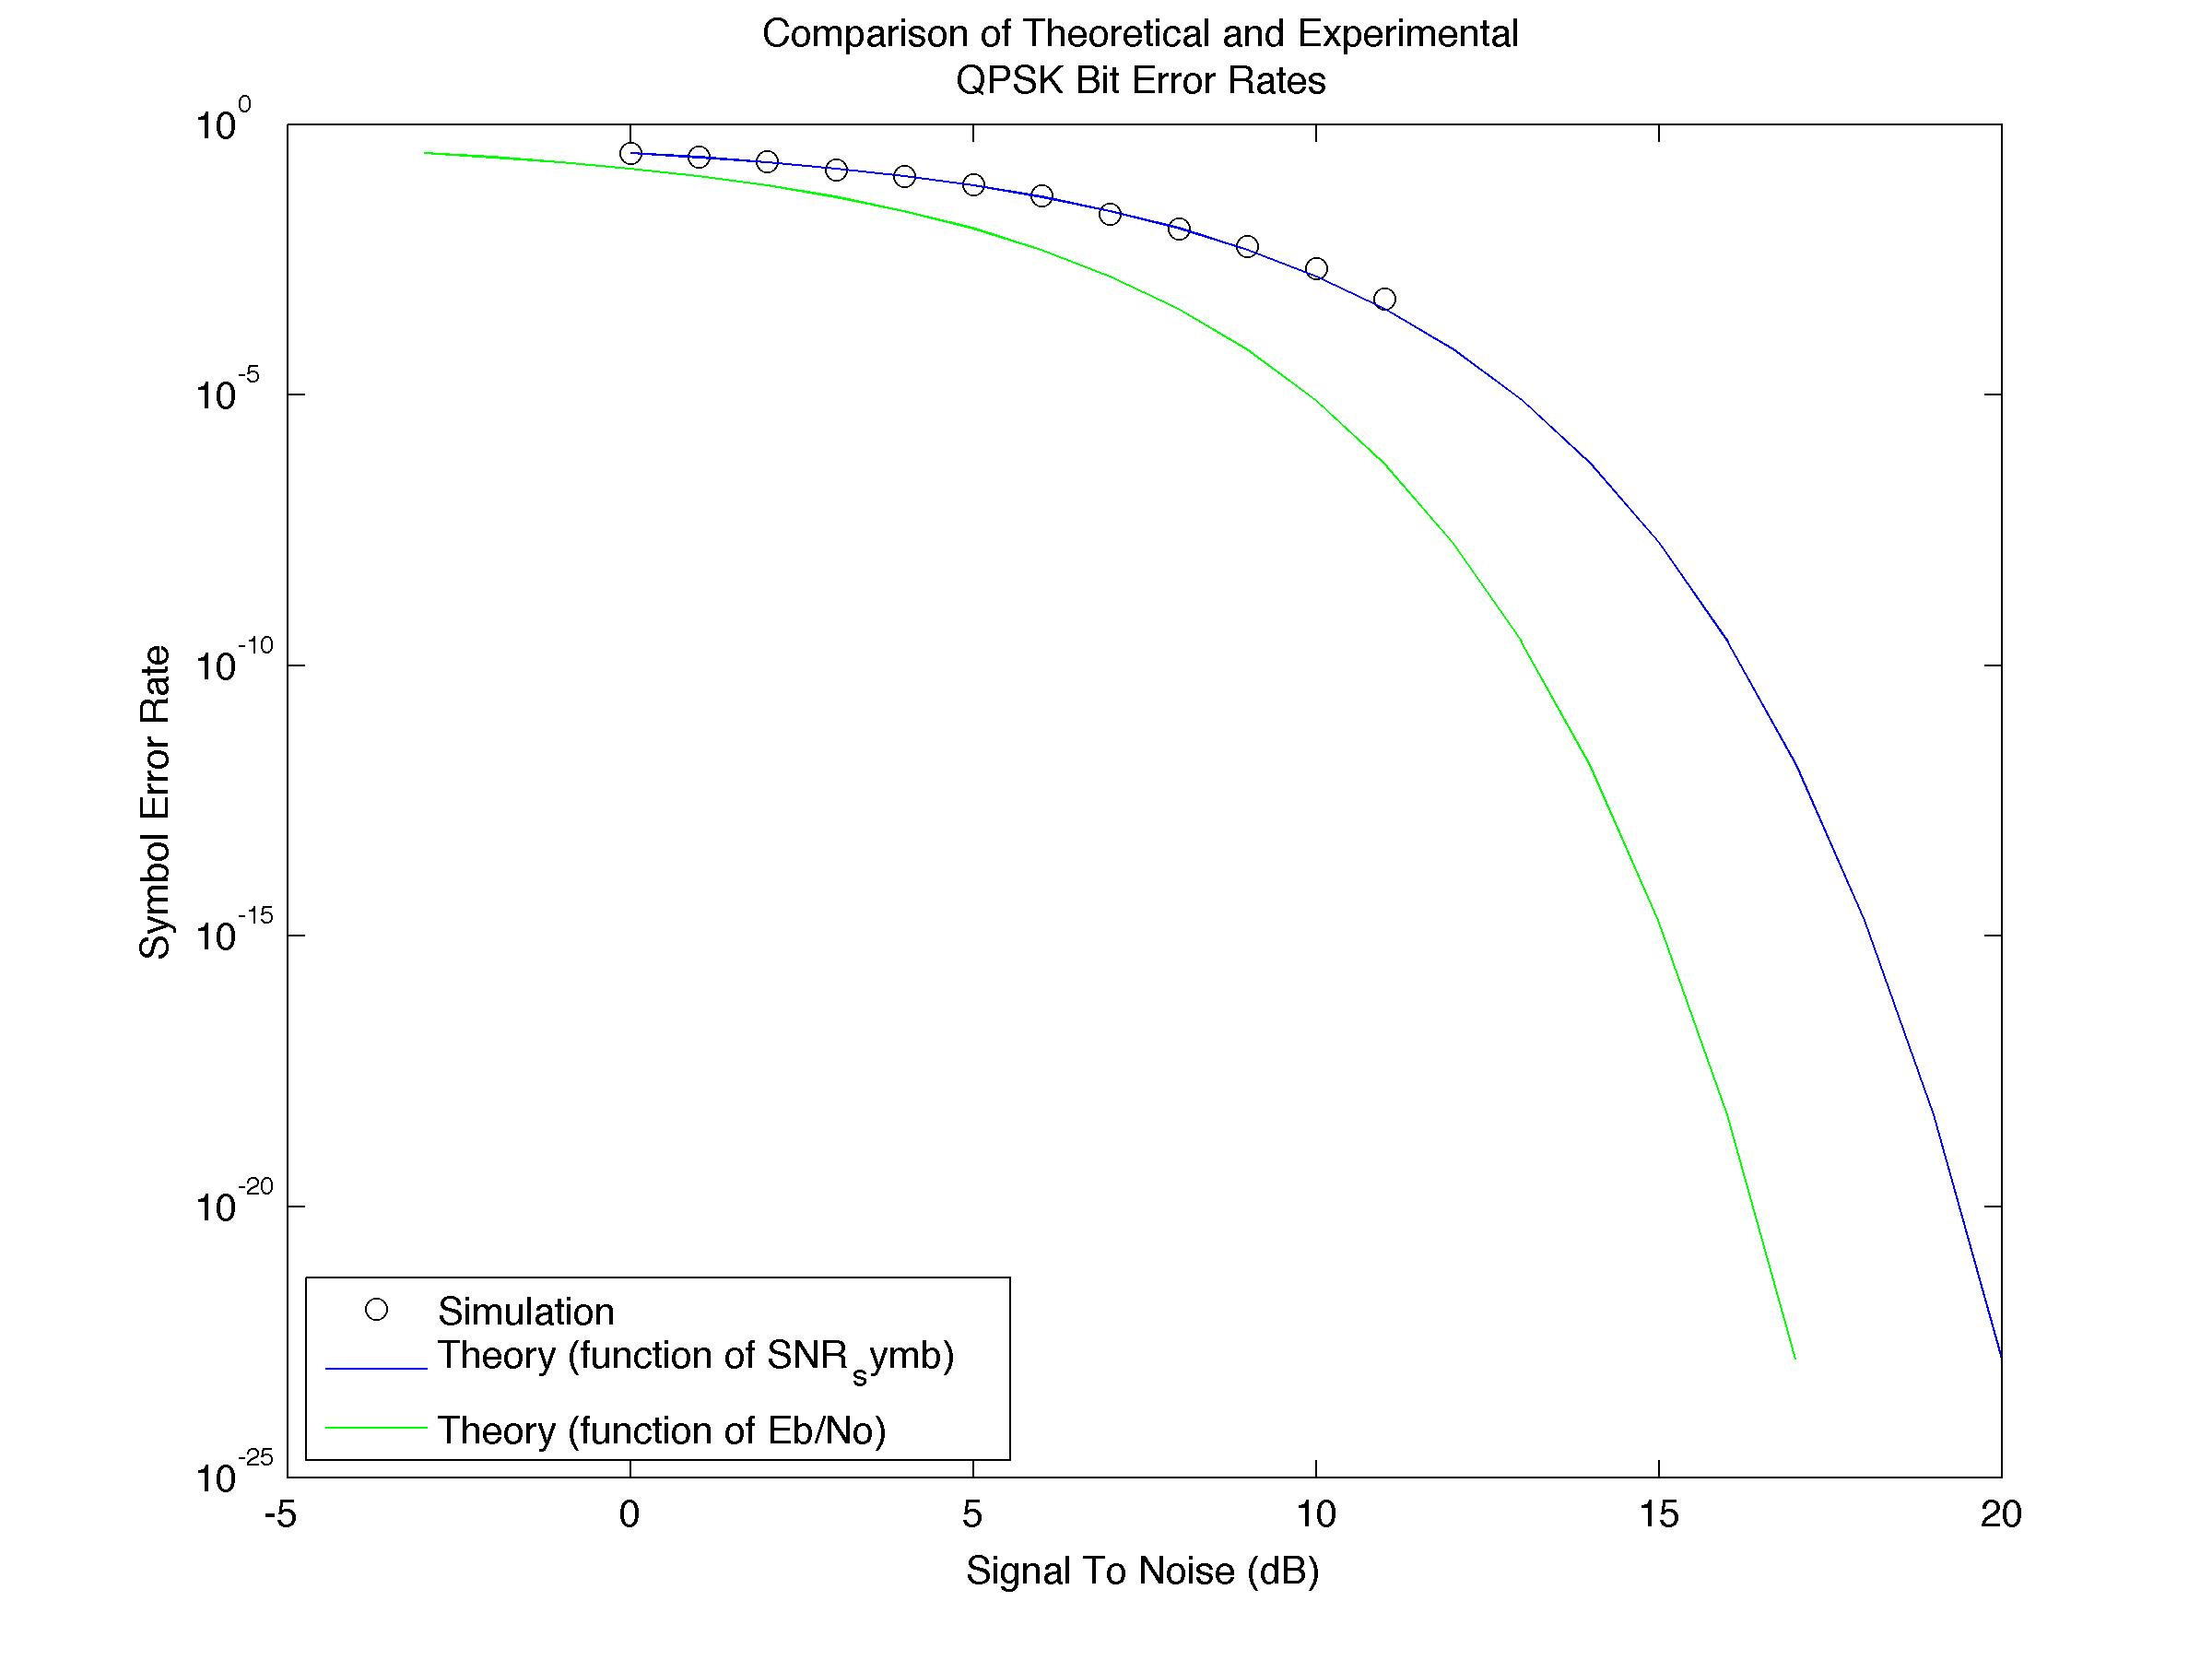
\includegraphics[width=1.3\textwidth]{qpSNR.jpg}
\caption{}
\end{figure}
\subsubsection{16-QAM}
\begin{figure}[H]
\centering
\hspace*{-2cm}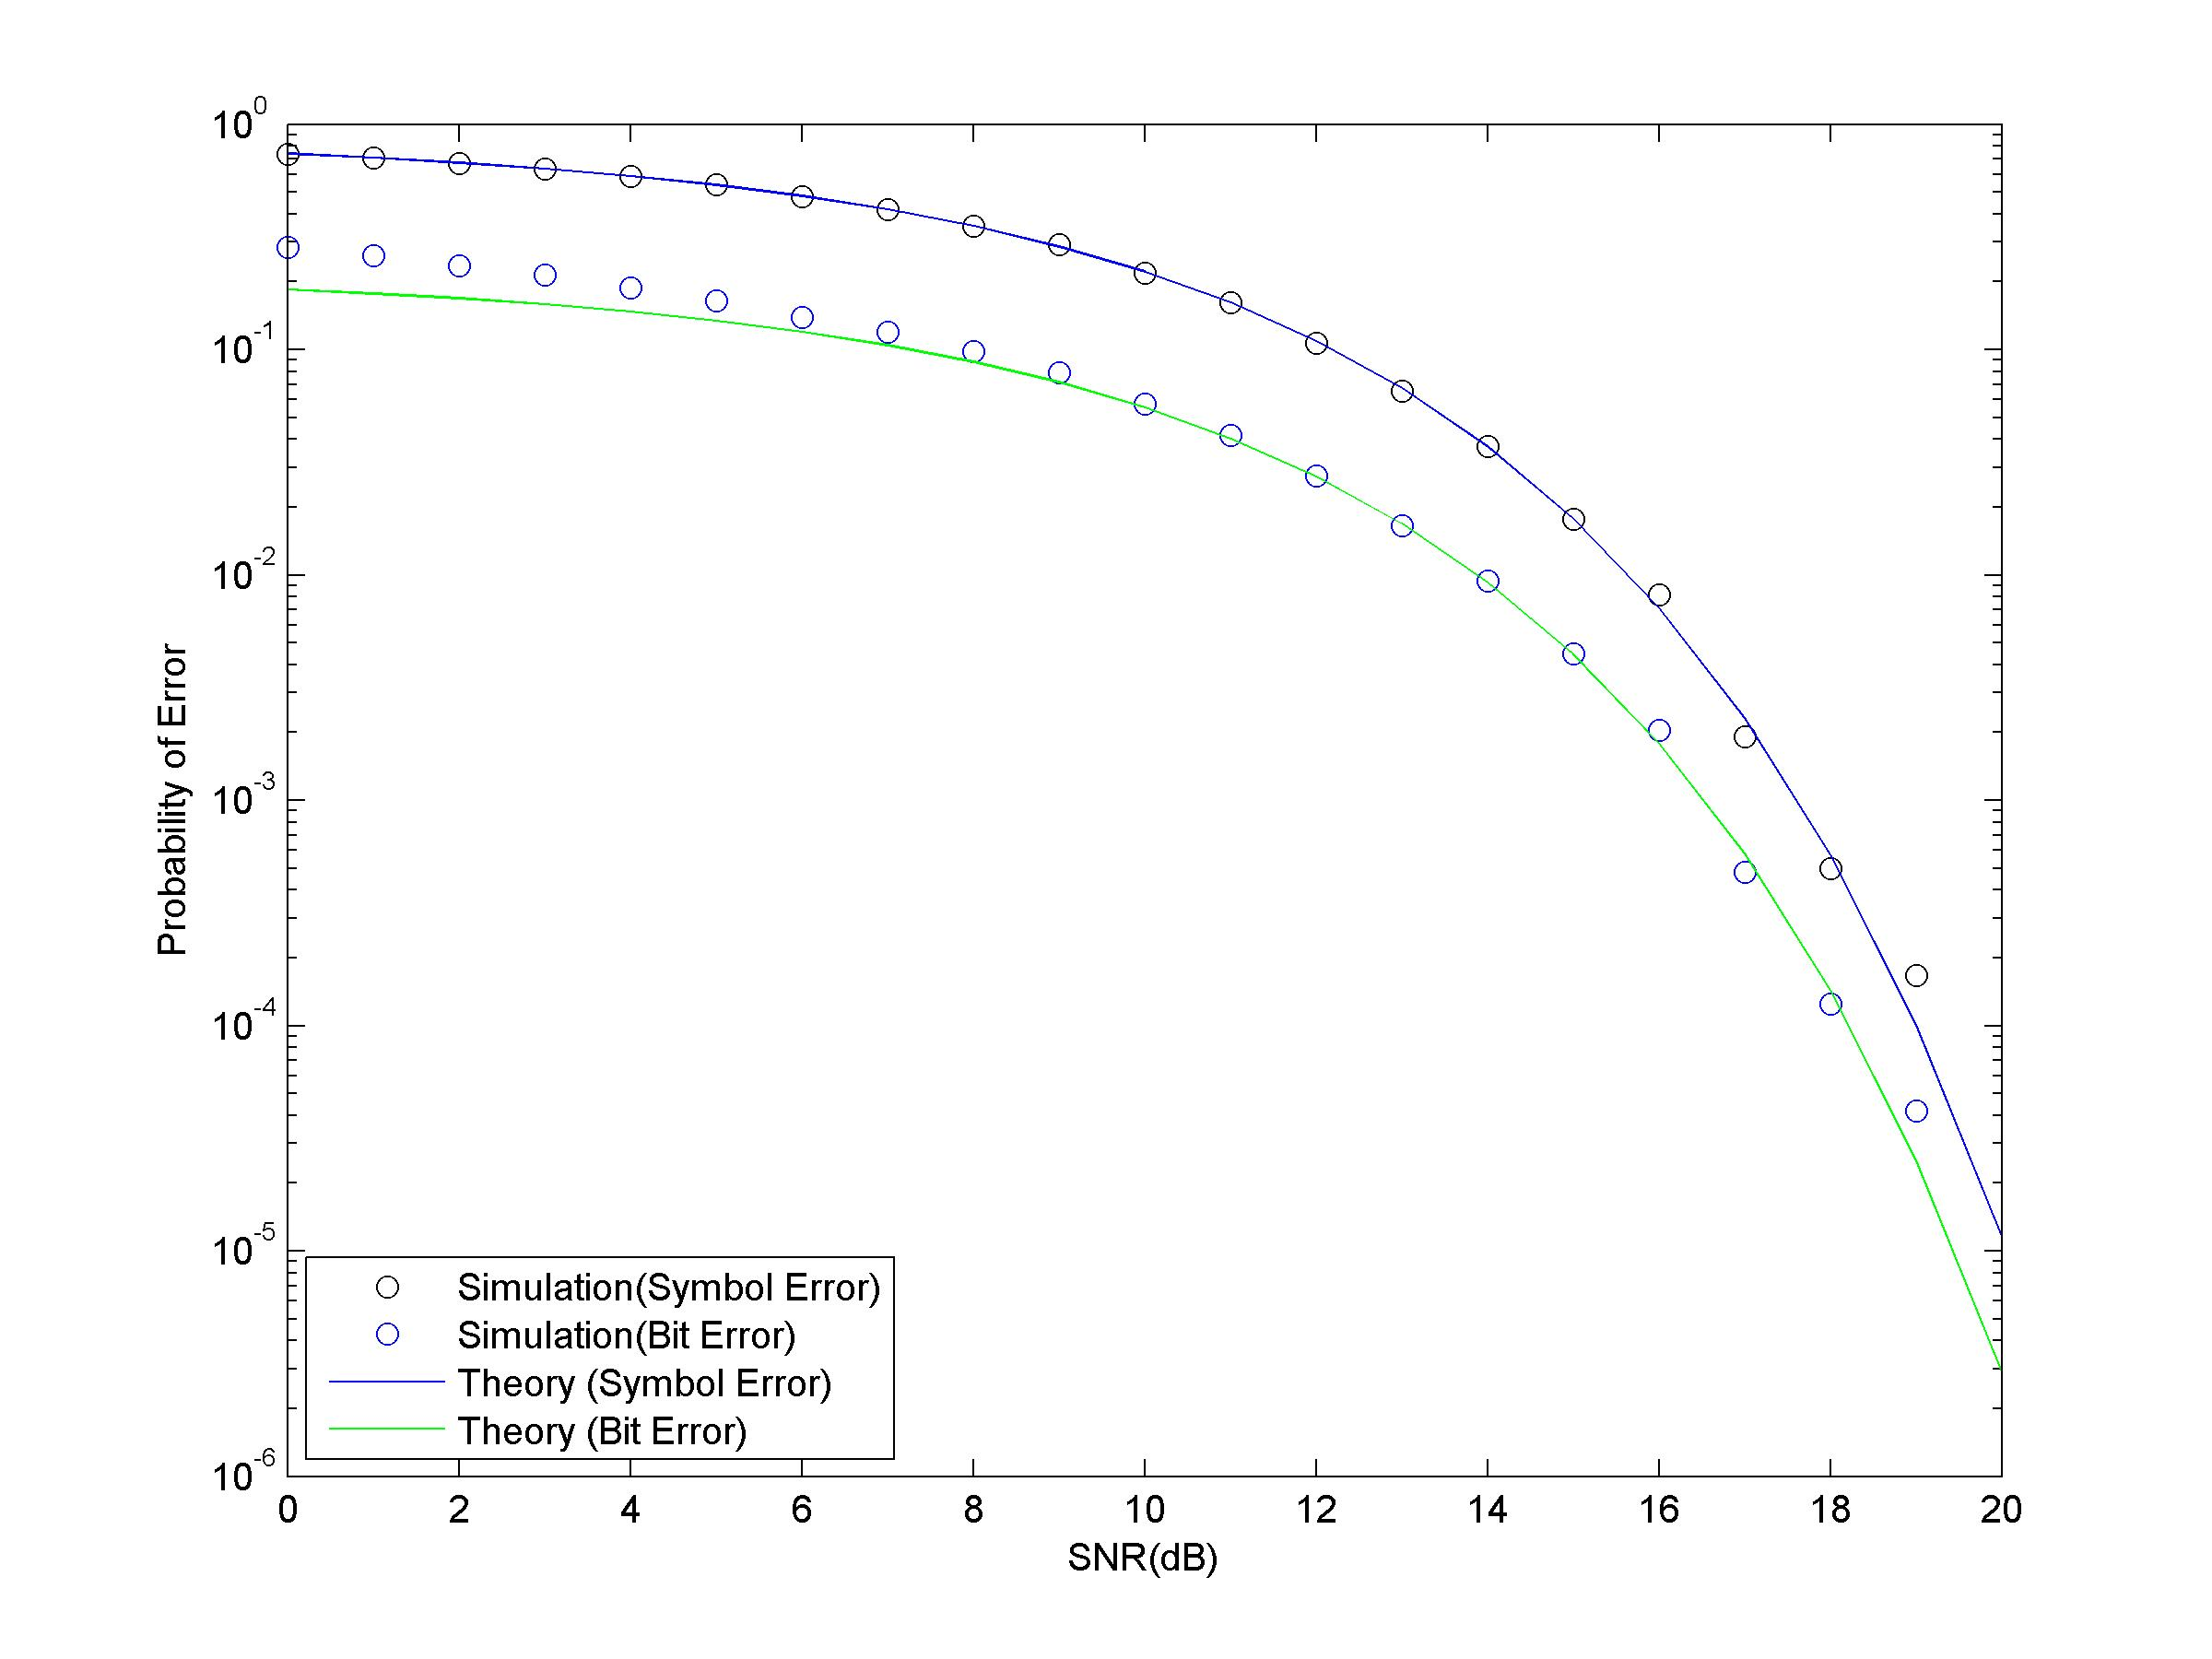
\includegraphics[width=1.3\textwidth]{qam16SNR.jpg}
\caption{}
\end{figure}
\subsubsection{64-QAM}
\begin{figure}[H]
\centering
\hspace*{-2cm}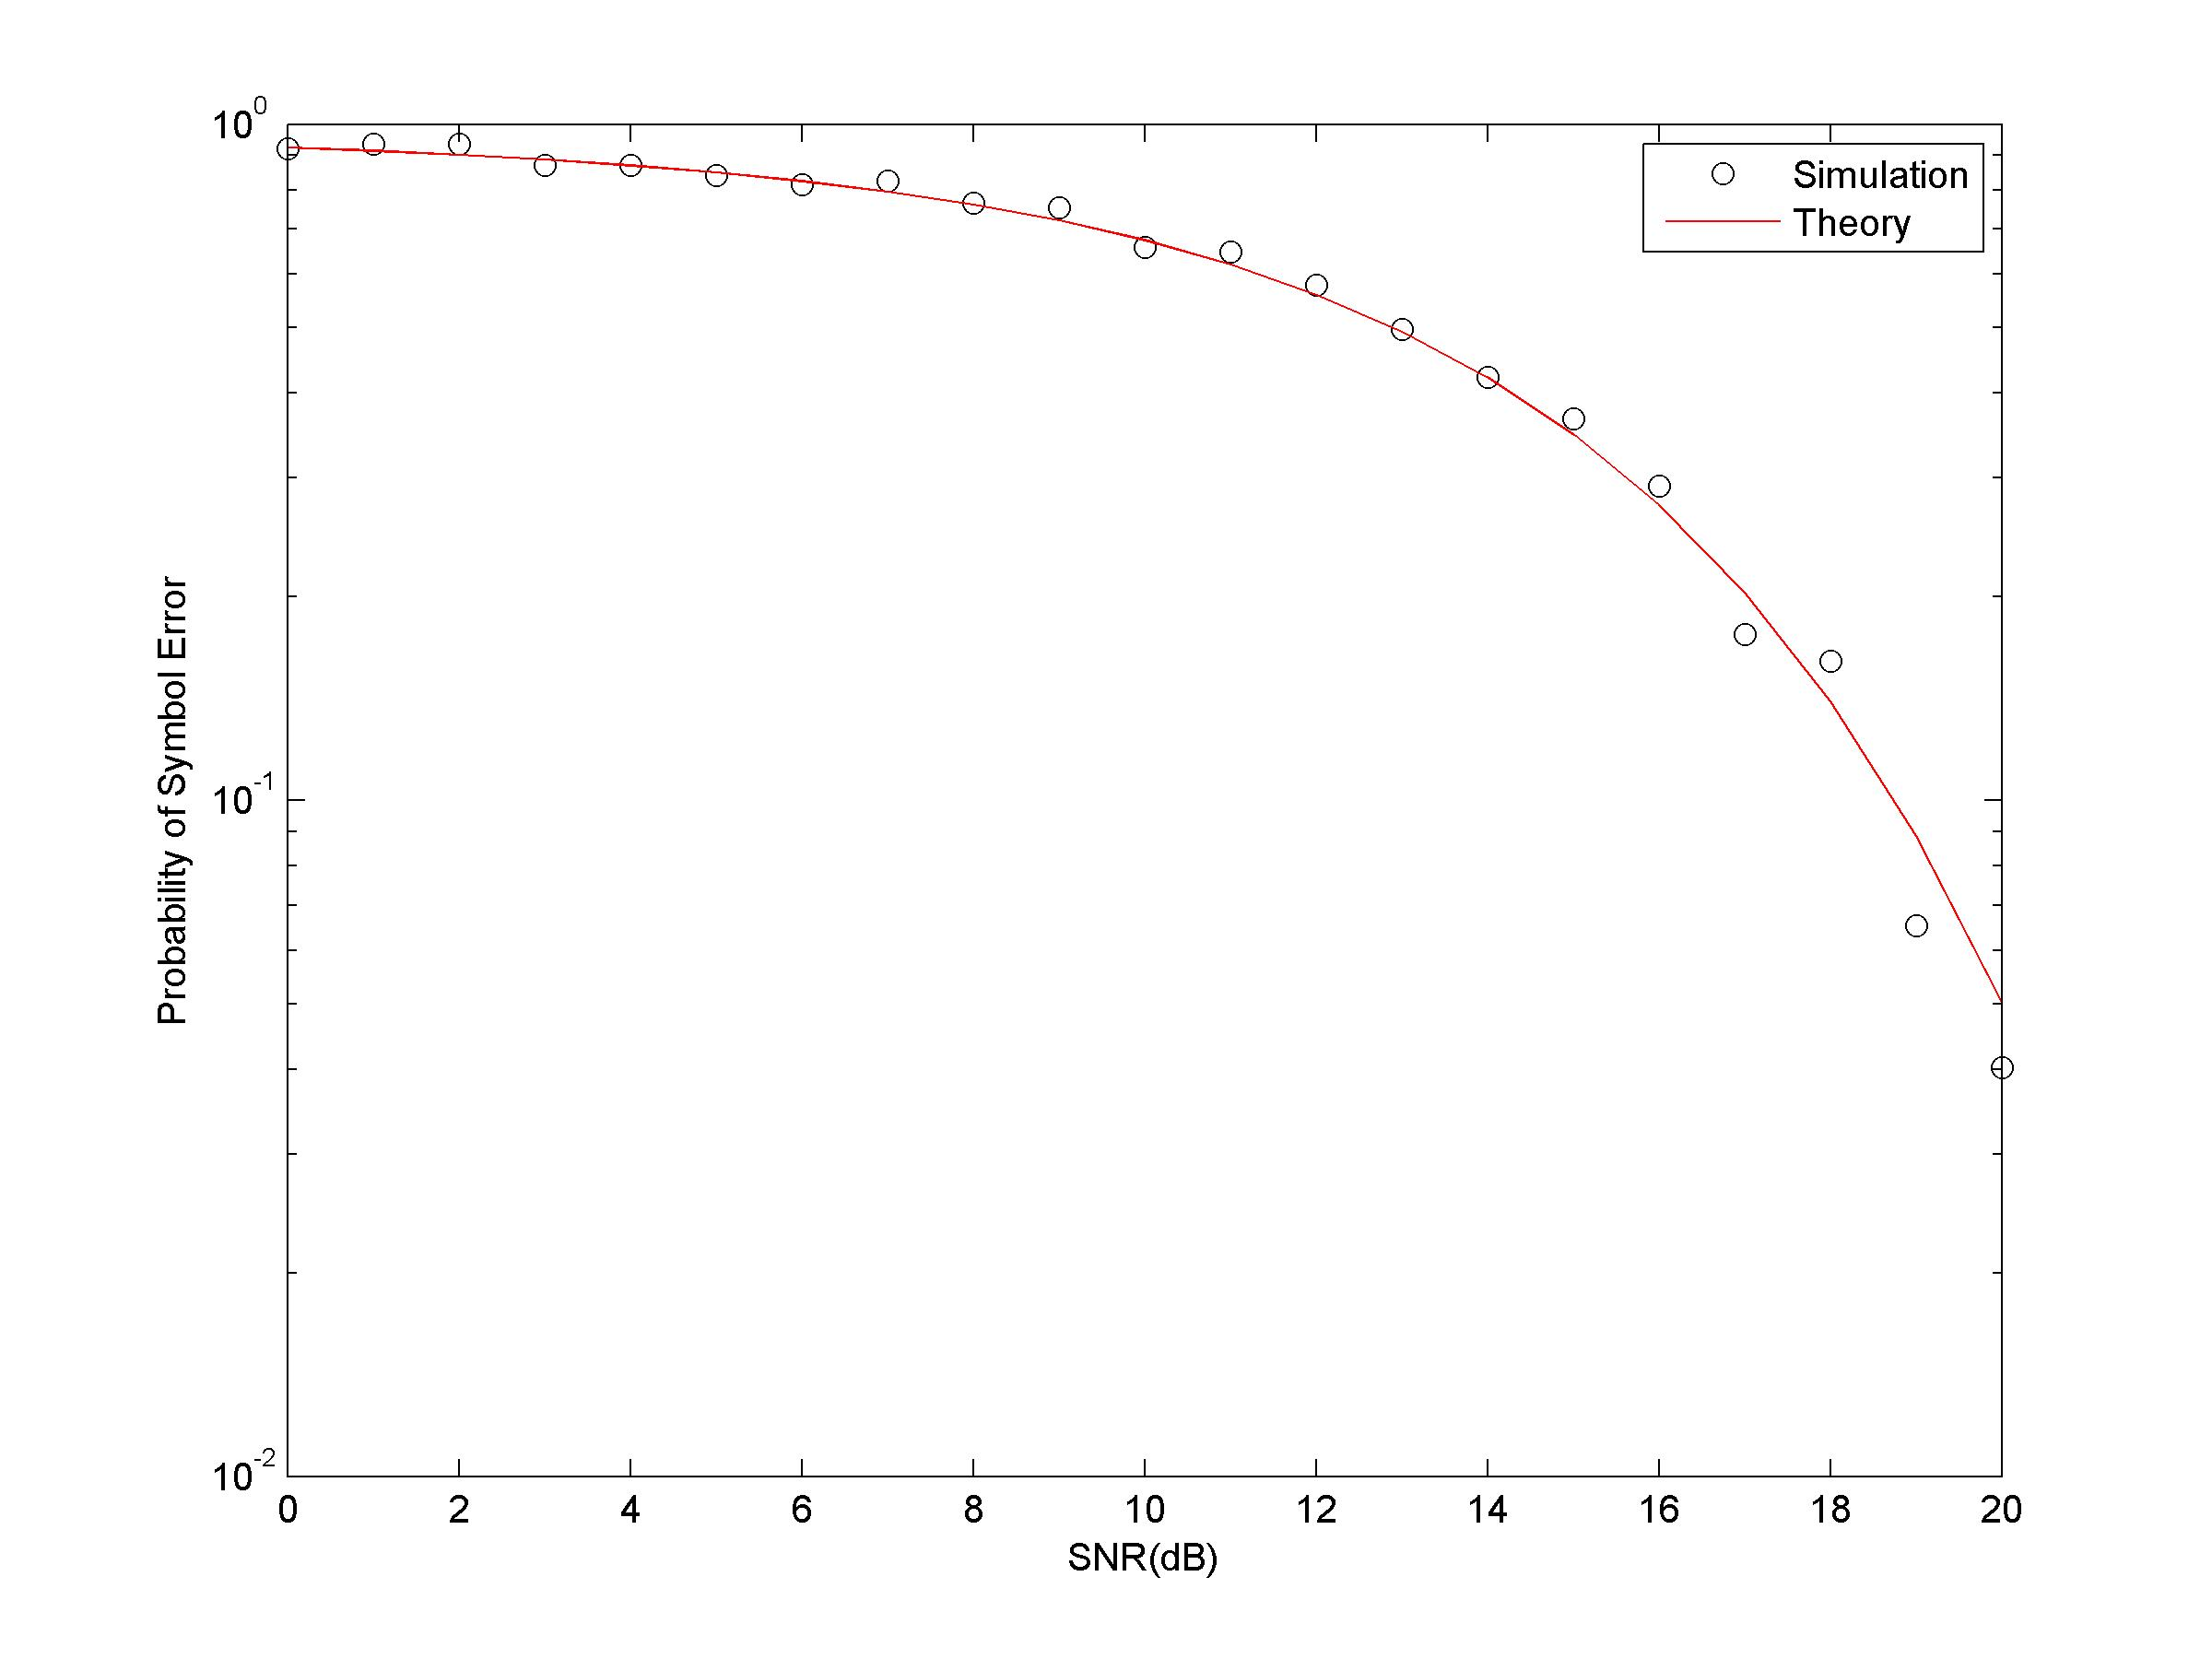
\includegraphics[width=1.3\textwidth]{qam64SNR.jpg}
\caption{}
\end{figure}
\subsection{Constellation Plots}
In the following sections scatter plots of BPSK, QPSK, 16-QAM and 64-QAM constellations are plotted at symbol/input SNRs of 3 dB, 6dB, 10dB and 20dB.

\subsubsection{BPSK}
\begin{figure}[H]
\centering
\hspace*{-2cm}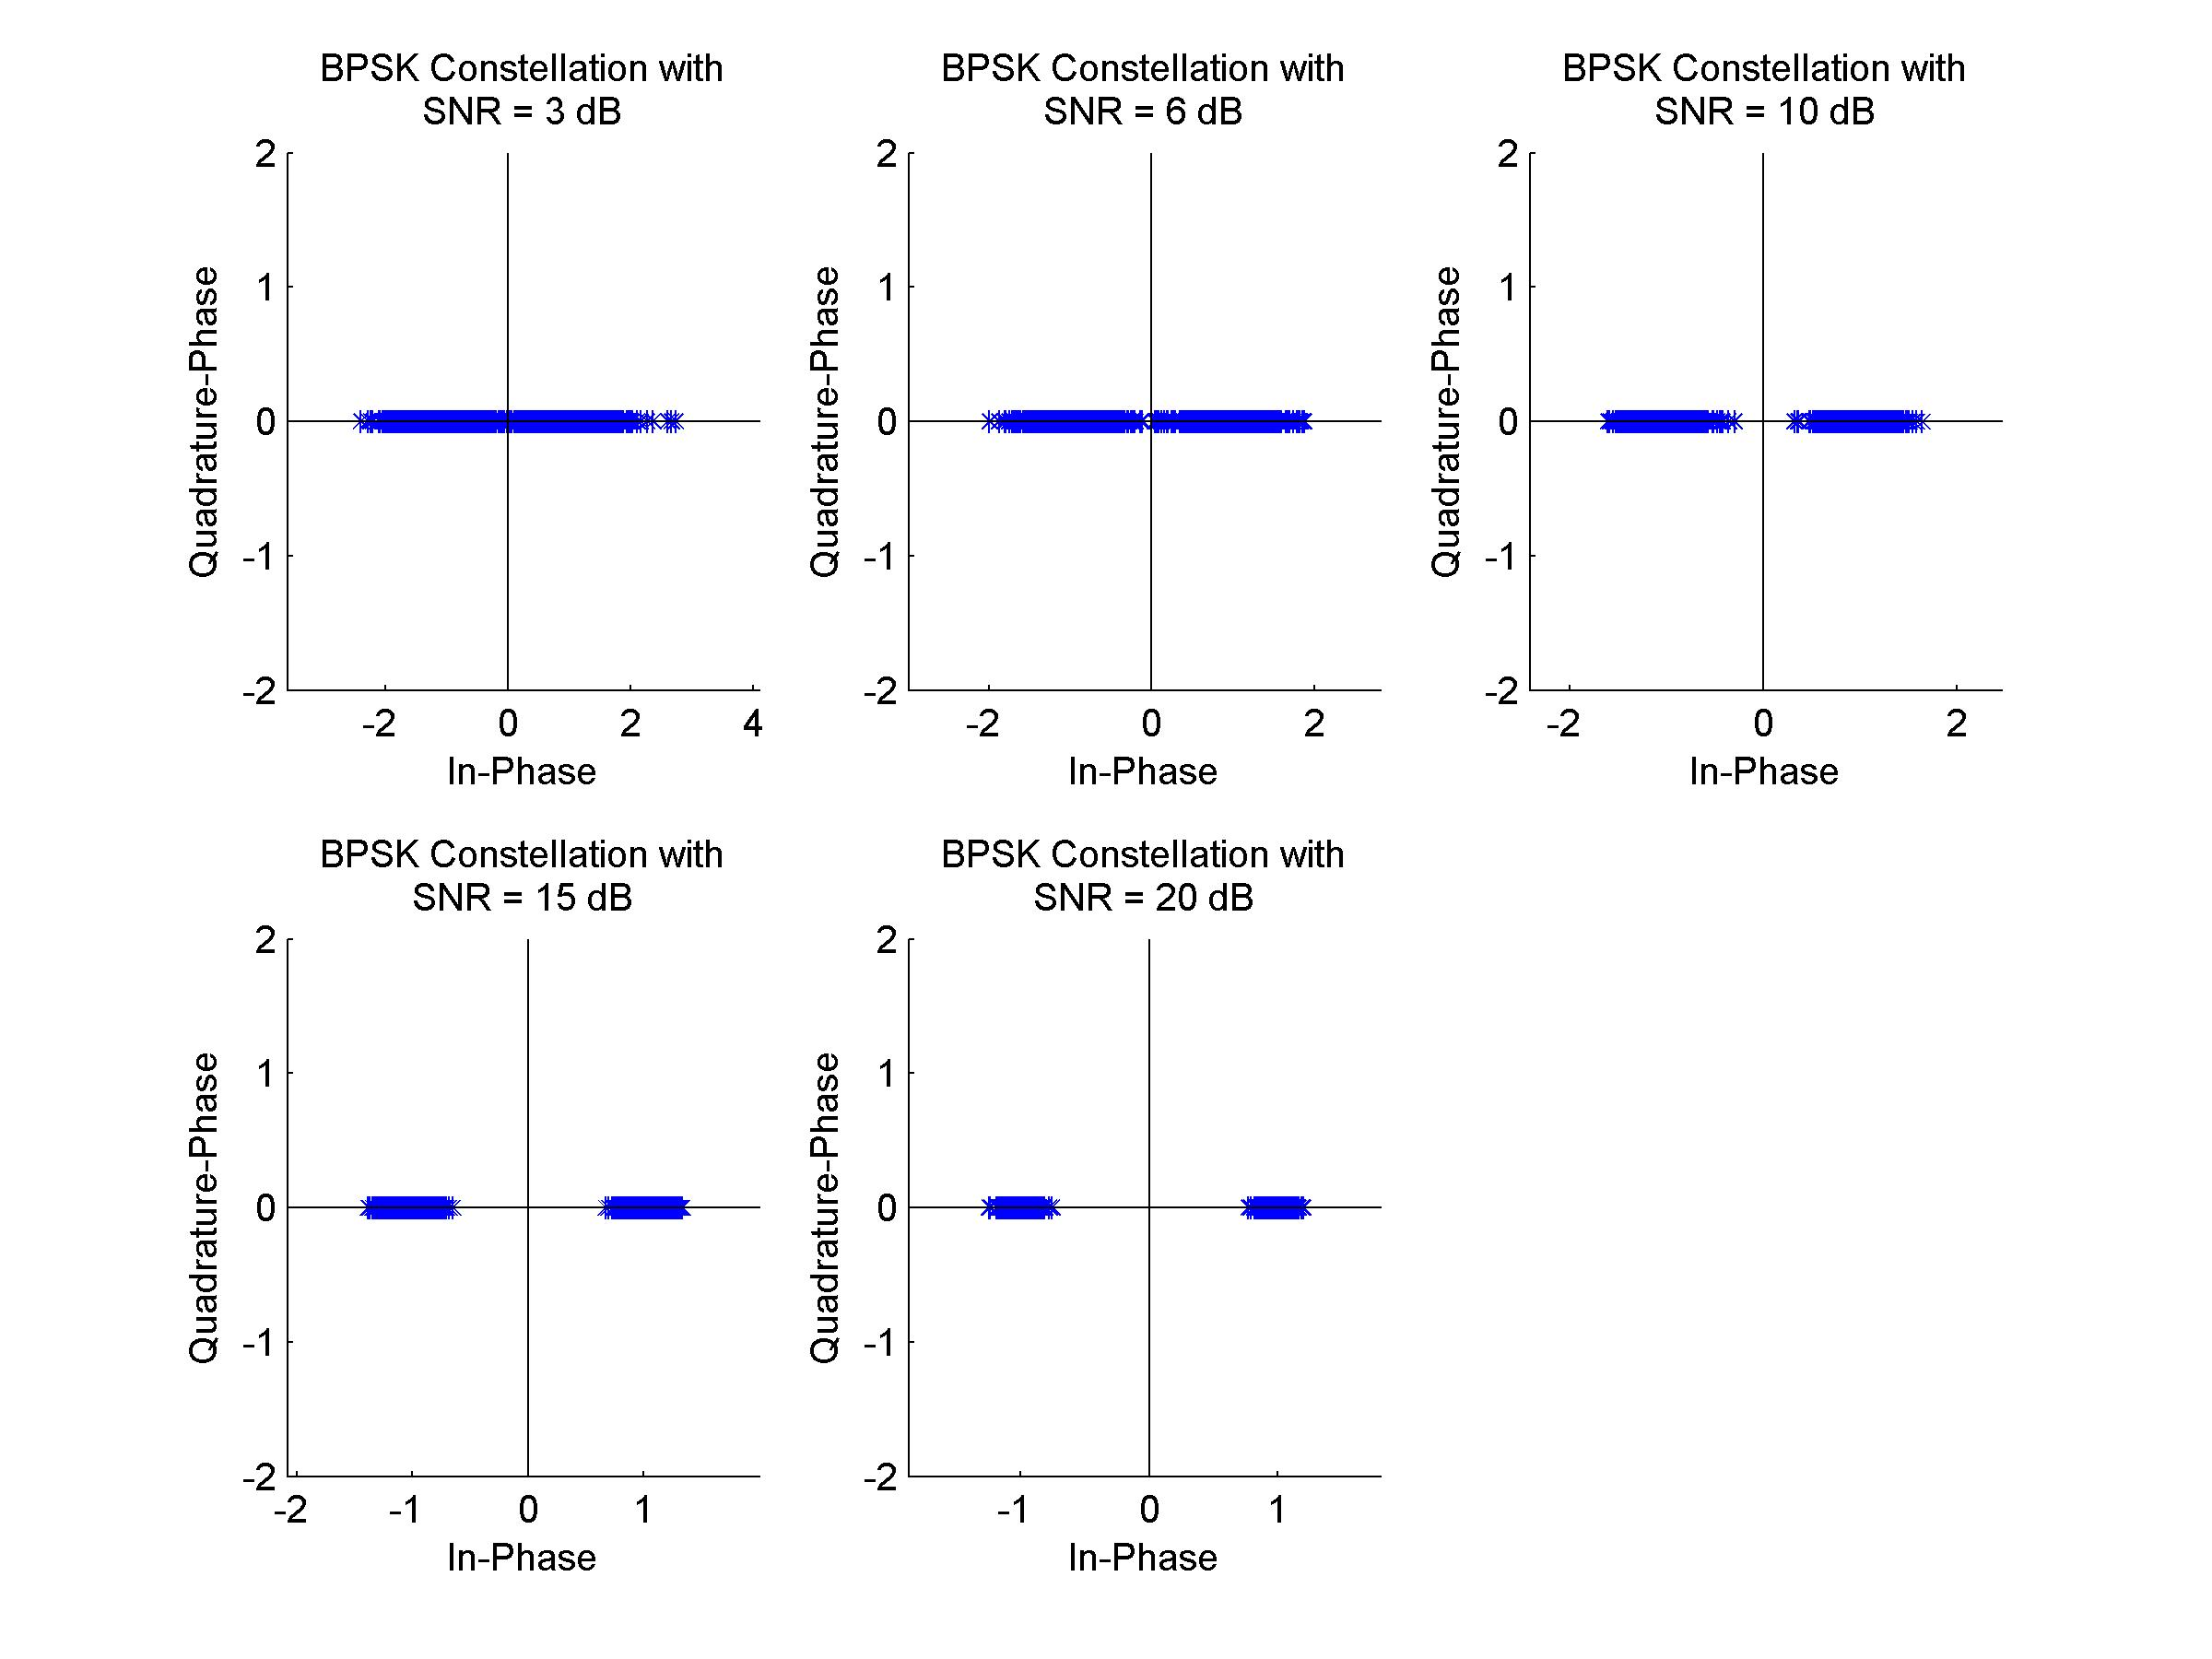
\includegraphics[width=1.3\textwidth]{bpConst.jpg}
\caption{}
\end{figure}
\subsubsection{QPSK}
\begin{figure}[H]
\centering
\hspace*{-2cm}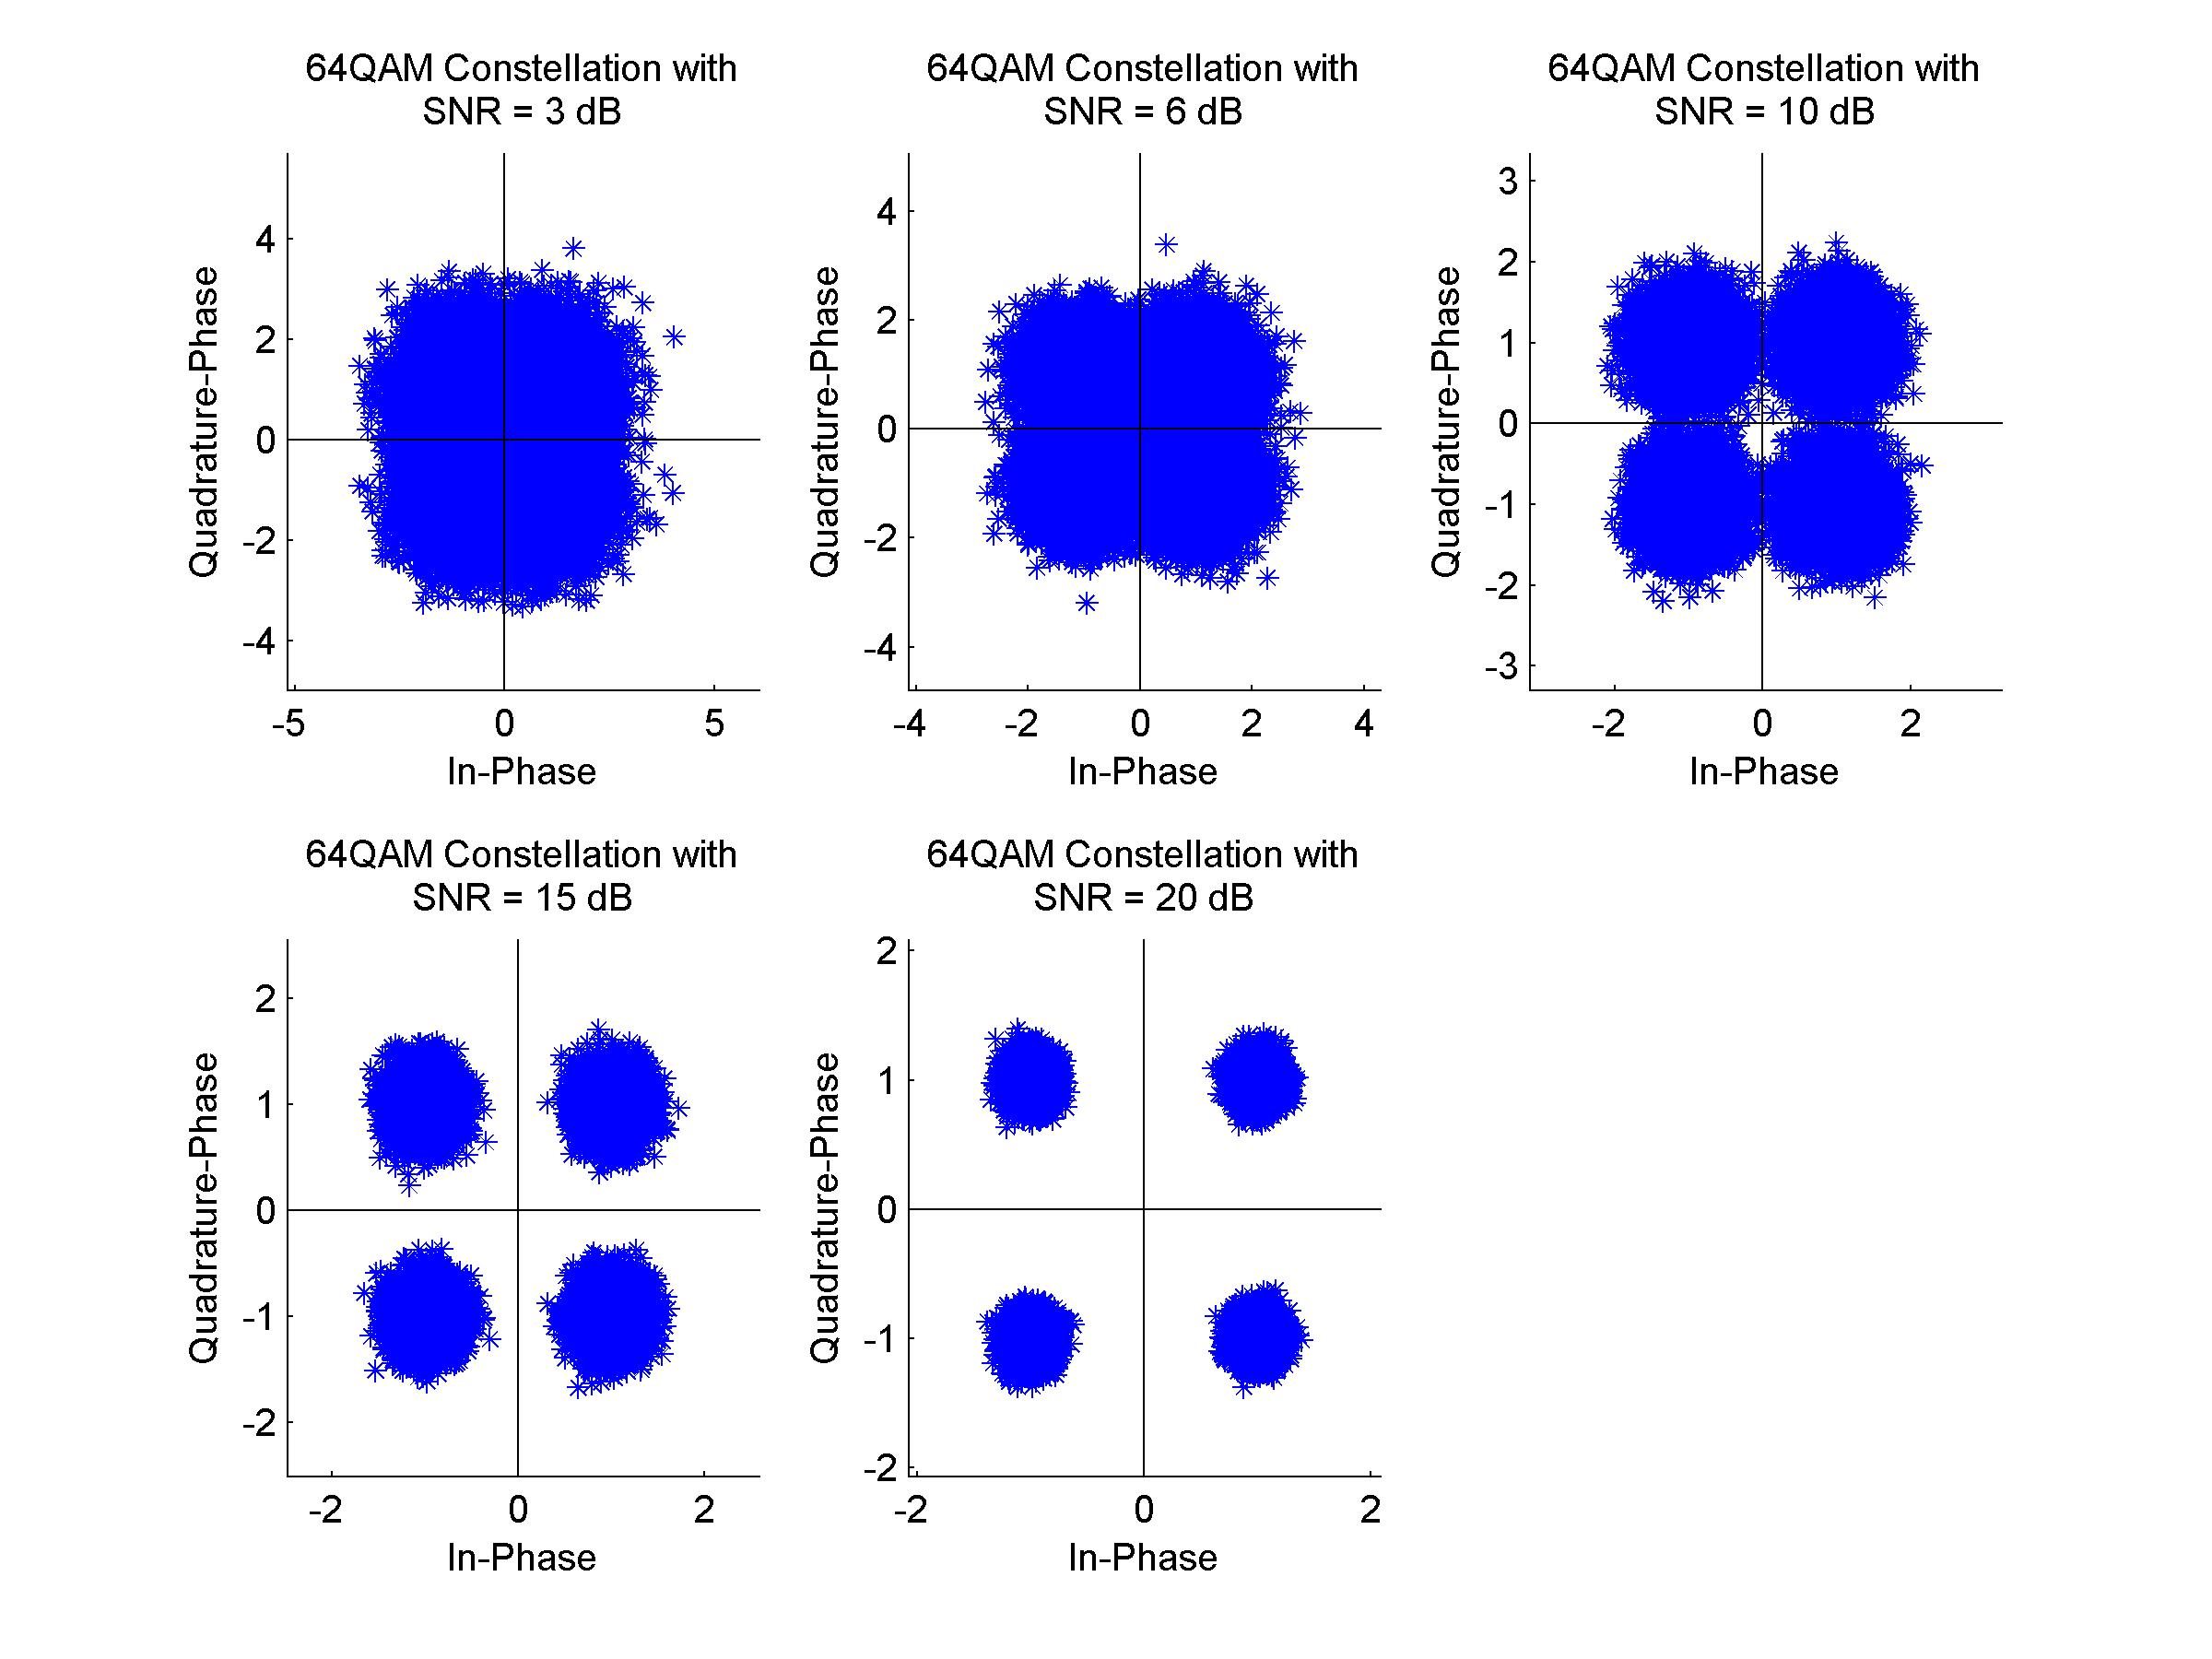
\includegraphics[width=1.3\textwidth]{qpConst.jpg}
\caption{}
\end{figure}
\subsubsection{16-QAM}
\begin{figure}[H]
\centering
\hspace*{-2cm}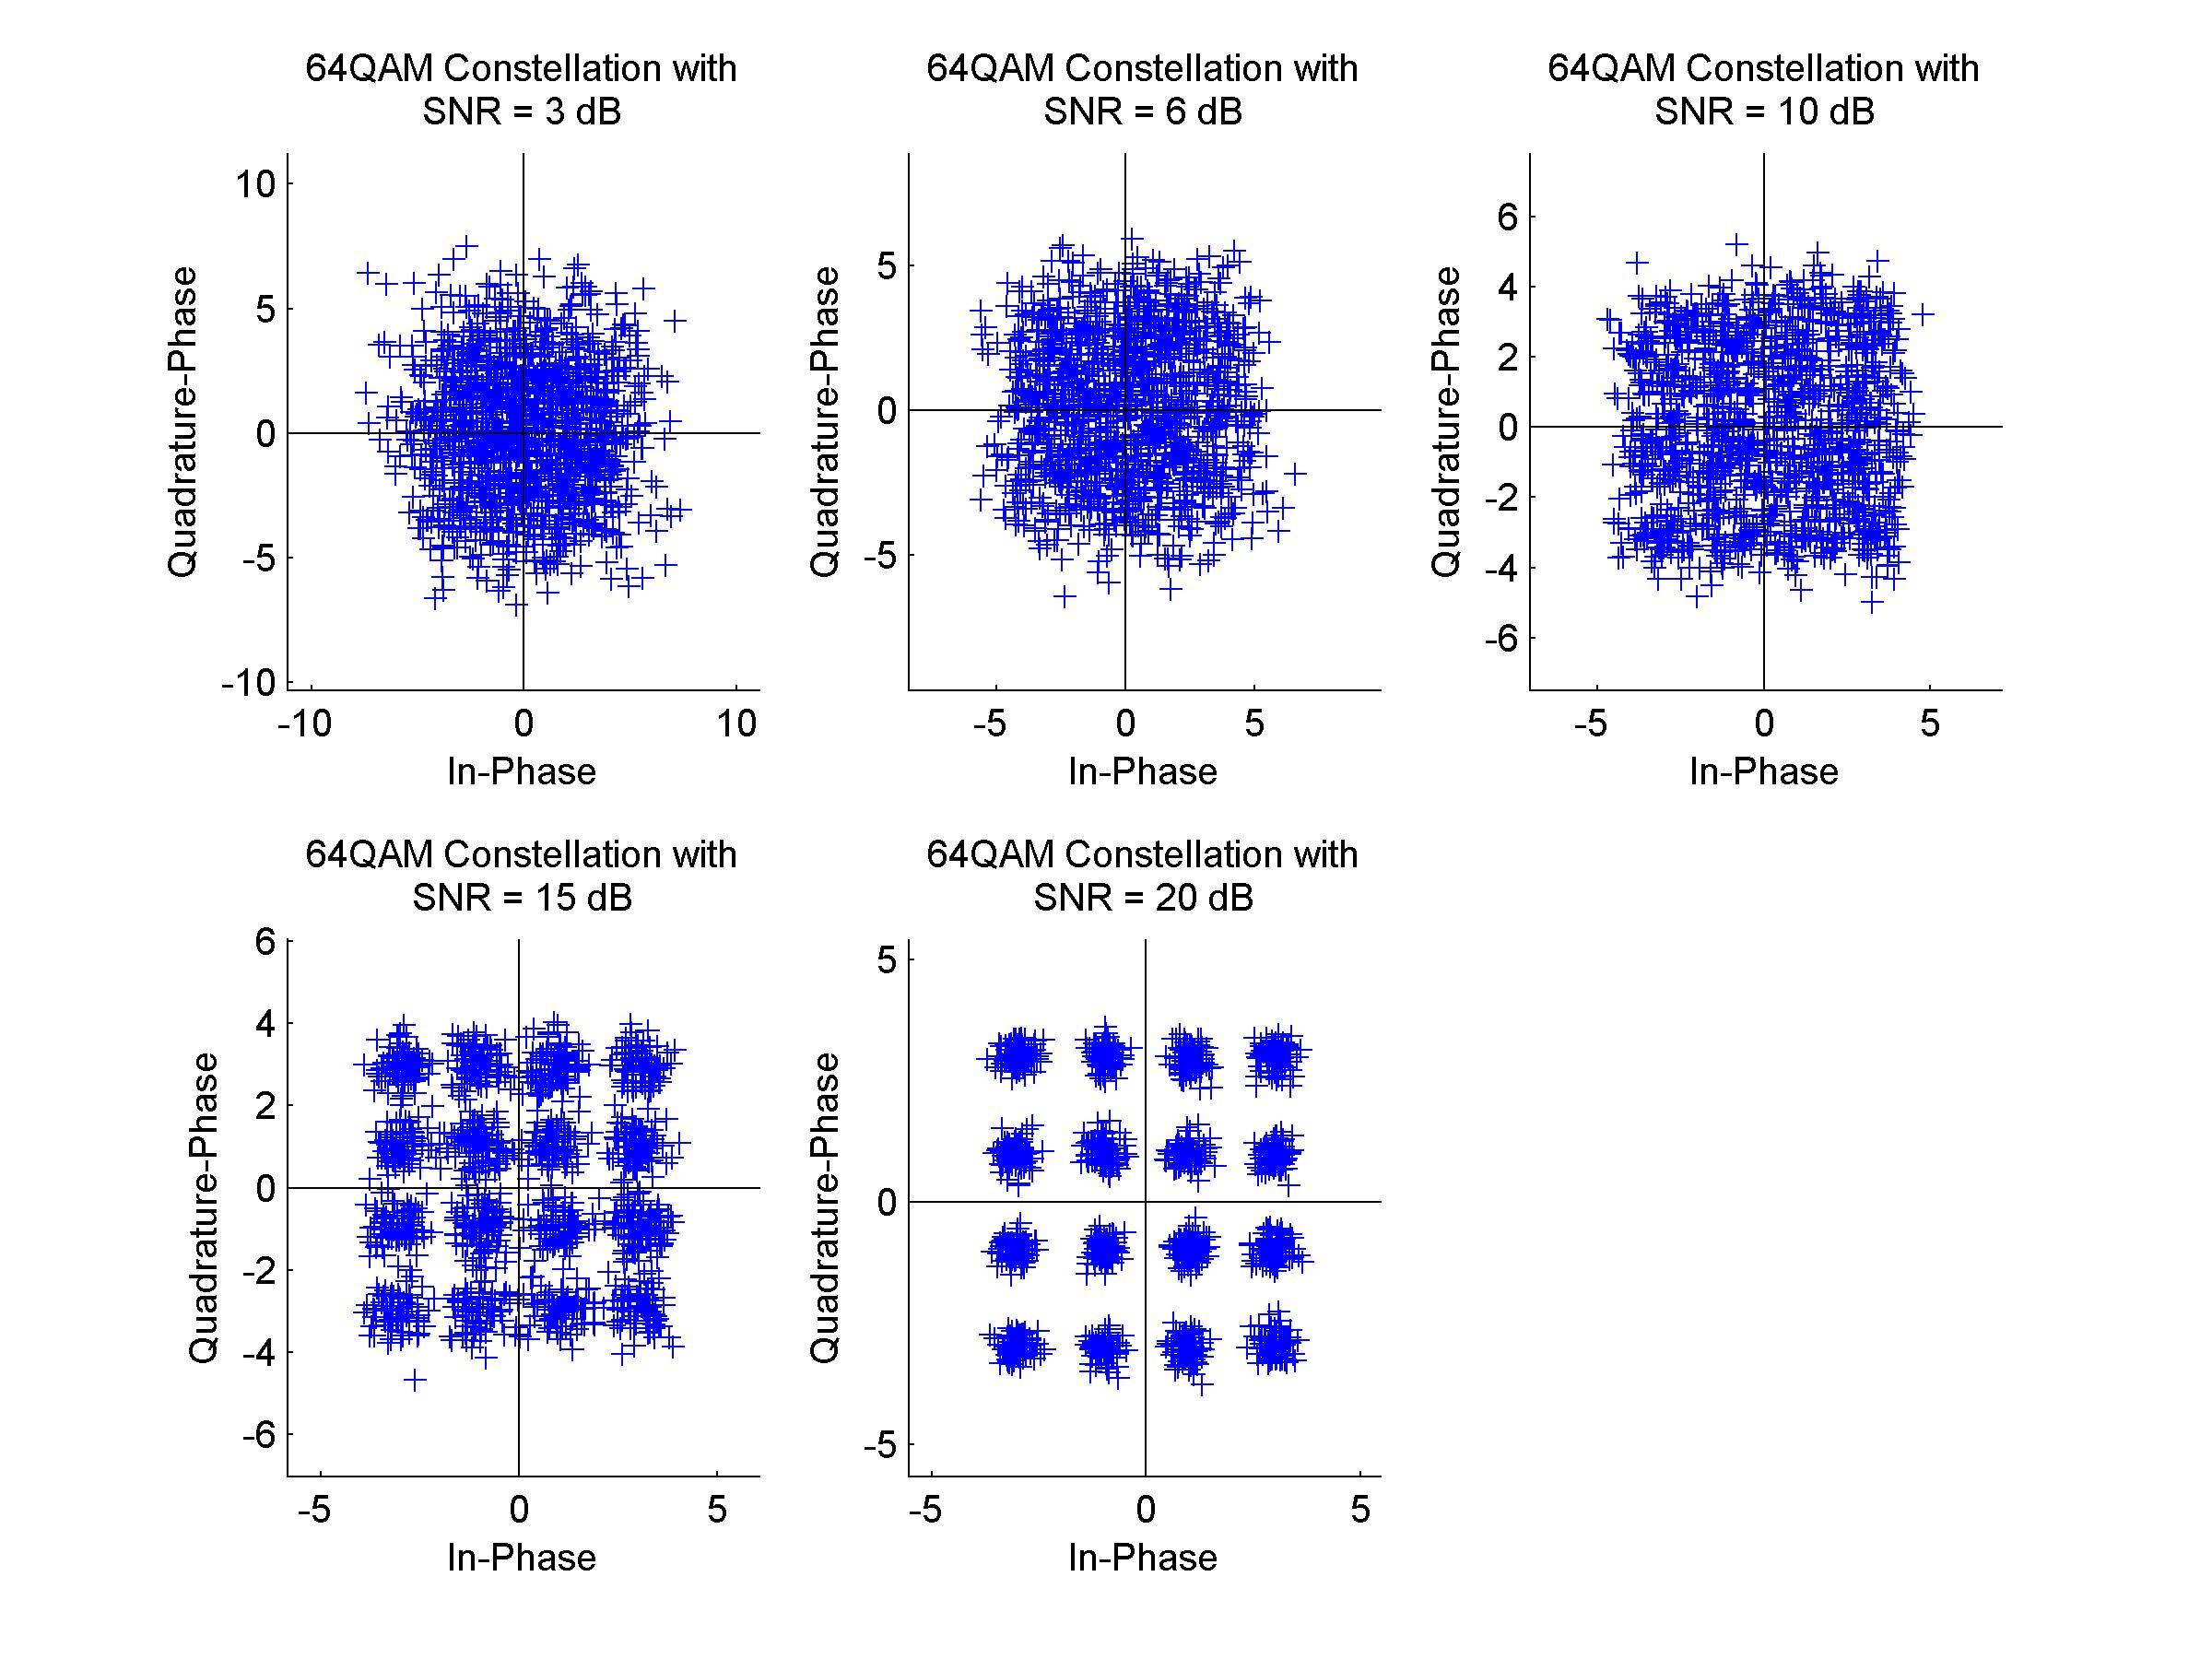
\includegraphics[width=1.3\textwidth]{qam16Const.jpg}
\caption{}
\end{figure}
\subsubsection{64-QAM}
\begin{figure}[H]
\centering
\hspace*{-2cm}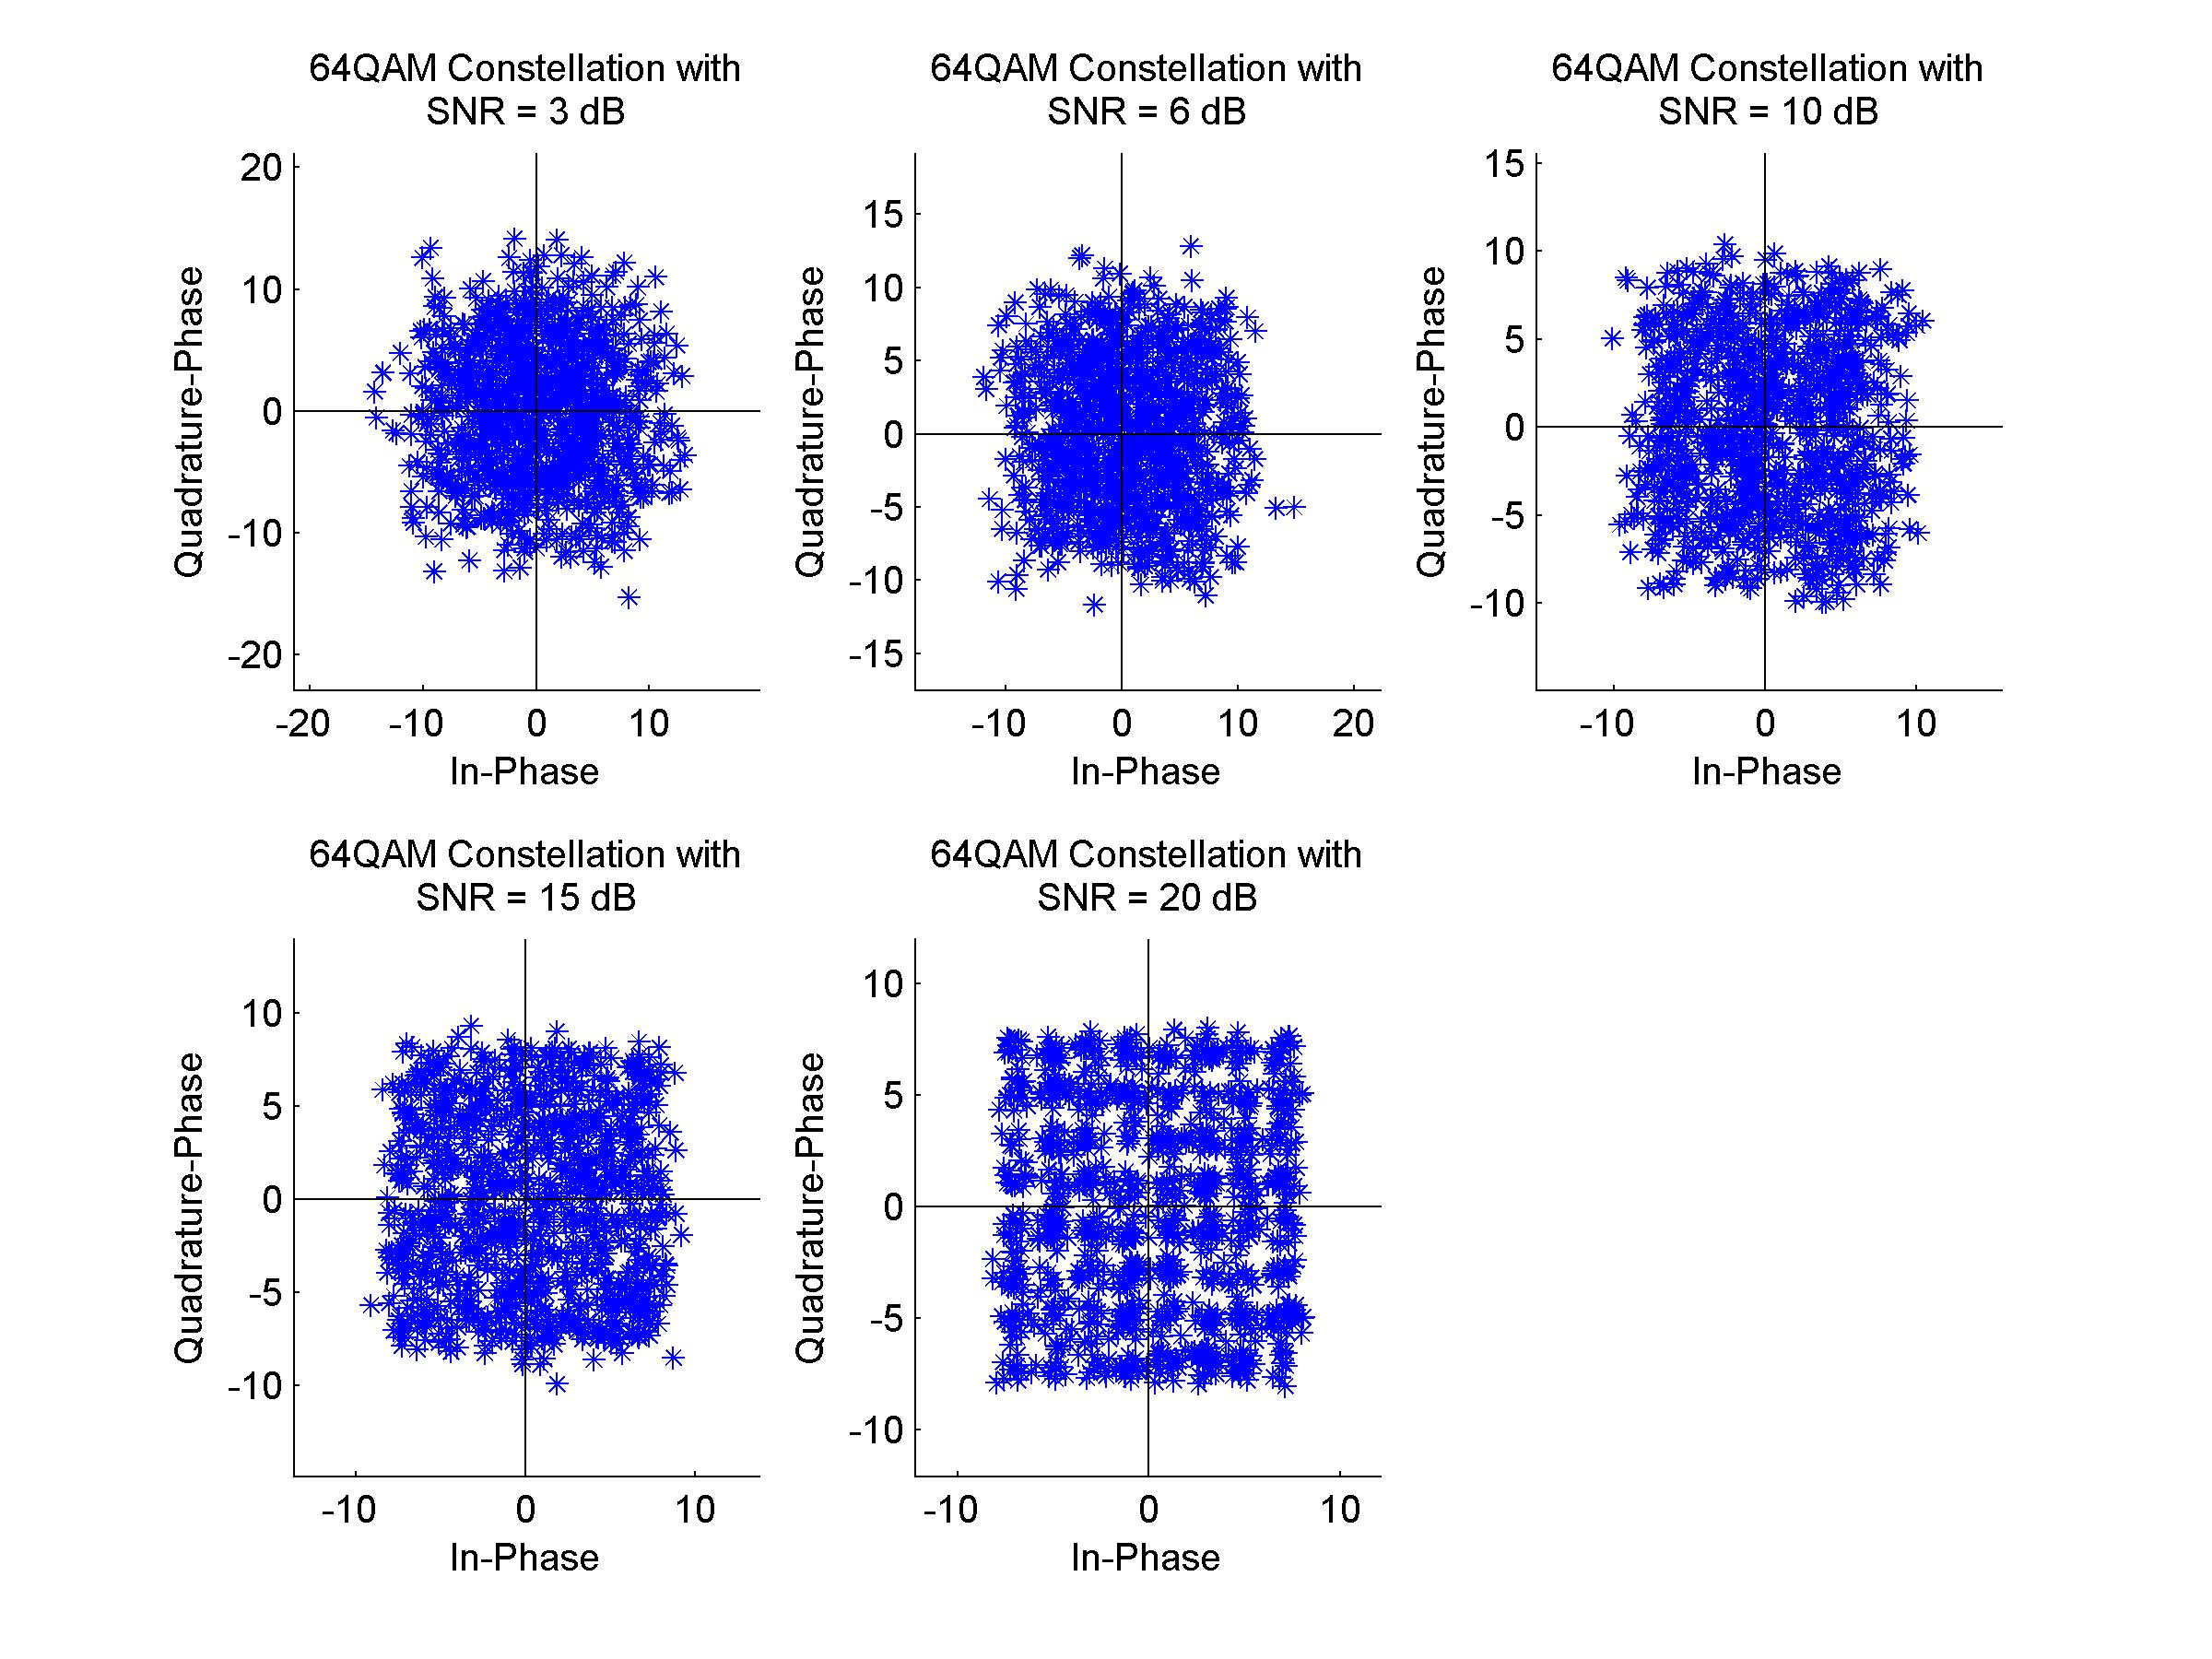
\includegraphics[width=1.3\textwidth]{qam64Const.jpg}
\caption{}
\end{figure}

\section{Conclusion}
\label{sec:conc}
This project was a demonstration of a digital communication with various modulation schemes.  The channel noise varied from tolerable to overpowering.  This can be seen in the both sets of plots.  These plots were made by sending 10,000 bits through the system and measuring the error rate.

\appendix
\newpage
%% the \\ insures the section title is centered below the phrase: Appendix B
%\section{Project Assignment}
%\label{app:assign}
%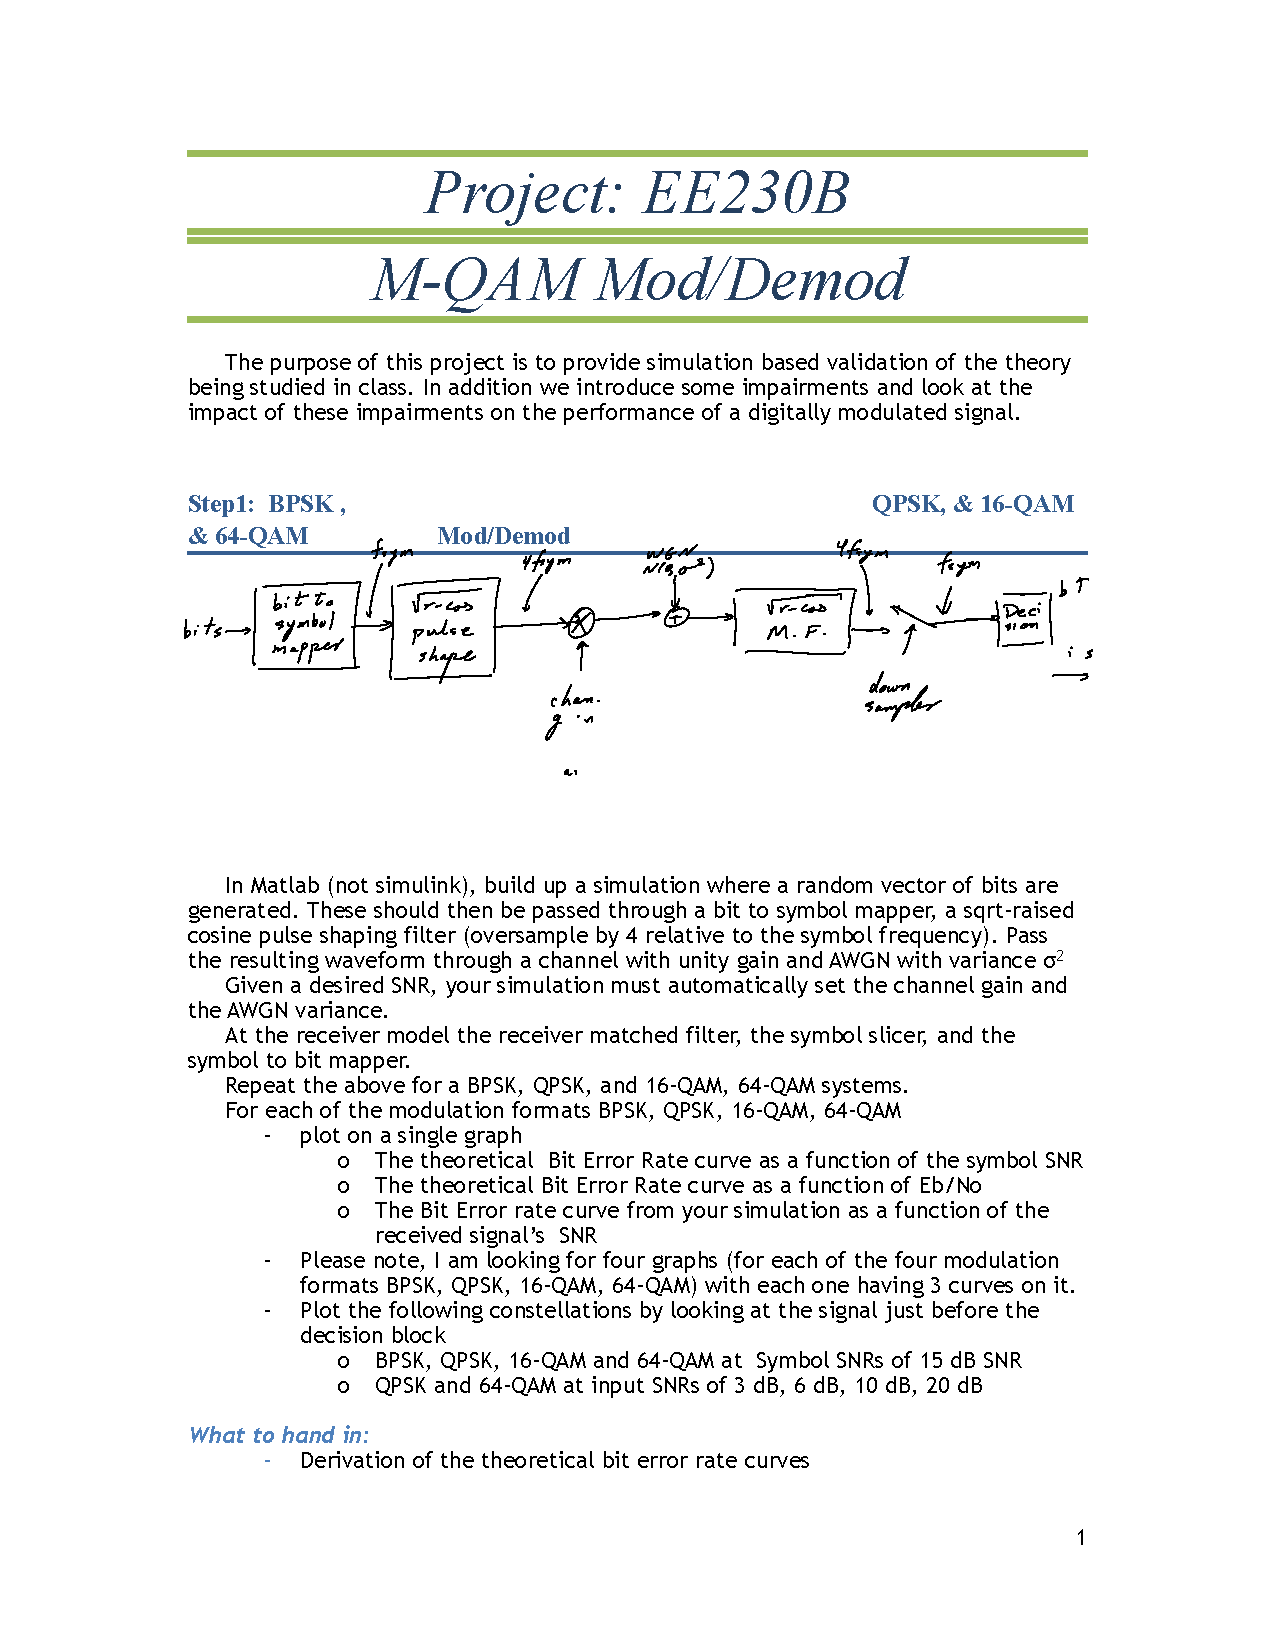
\includepdf[pages={1-5}]{project_overview.pdf}
%\cleardoublepage
%\newpage


\section{Random Bit Sequence Generator}
\label{app:random_bit_generator}
\lstinputlisting{random_bit_generator.m}
\cleardoublepage
\newpage

\section{Bit to Symbol Mappers}
\label{app:bittosym}
\subsection{BPSK Modulation }
\label{app:bpsk_mod}
% To convert program (e.g. C++ Fortran, Matlab, LaTeX) listings to a
% form easily includable in a LaTeX document
%
% type lgrind -s to see options
% lgrind -llatex -i sample-paper.tex > sampleinputtex
% creates a file sampleinput.tex which can then be included into this
% document simply by uncommenting the next line
%\lgrindfile{testinput.tex}

\lstinputlisting{bpsk_mod.m}
\cleardoublepage  % force onto odd page
\newpage

\subsection{QPSK Modulation}
\label{app:qpsk_mod}
\lstinputlisting{qpsk_mod.m}
\cleardoublepage  % force onto odd page
\newpage

\subsection{16-QAM Modulation}
\label{app:qam_16_mod}

\lstinputlisting{QAM_16_mod.m}
\cleardoublepage  % force onto odd page
\newpage

\subsection{64-QAM Modulation }
\label{app:qam_64_mod}
\lstinputlisting{QAM_64_mod.m}
\cleardoublepage  % force onto odd page
\newpage

\section{Square Root Raised Cosine Filter}
\label{app:sqrt_raised_cosine}
\lstinputlisting{sqrt_raised_cosine.m}
\cleardoublepage
\newpage

\section{Up Sampler}
\label{app:impulse_train}
\lstinputlisting{impulse_train.m}
\cleardoublepage
\newpage

\section{Additive Gaussian White Noise Channel}
\label{app:awgn_channel}
\lstinputlisting{awgn_channel.m}
\cleardoublepage
\newpage

\section{Additive Gaussian White Noise Channel}
\label{app:awgn_channel}
\lstinputlisting{awgn_channel.m}
\cleardoublepage
\newpage

\section{Sampler}
\label{app:sampler}
\lstinputlisting{sampler.m}
\cleardoublepage
\newpage

\section{Decision Blocks}
\label{app:dblocks}
\subsection{BPSK Demodulation}
\label{app:bpsk_demod}
\lstinputlisting{bpsk_demod.m}
\cleardoublepage
\newpage

\subsection{QPSK Demodulation}
\label{app:qpsk_demod}
\lstinputlisting{qpsk_demod.m}
\cleardoublepage
\newpage

\subsection{16-QAM Demodulation}
\label{app:qam_16_demod}
\lstinputlisting{QAM_16_demod.m}
\cleardoublepage
\newpage

\subsection{64-QAM Demodulation}
\label{app:qam_64_demod}
\lstinputlisting{QAM_64_demod.m}
\cleardoublepage
\newpage


\end{document}